%!TEX root = TDT4265-Summary.tex
\section{Representation and description}
The results of image segmentation (Section \ref{sec:segmentation}) can be represented and described in certain ways to be useful for computers. For instance, a region can be represented by its boundary, and the boundary described by its lenght.

%%%%%%%%%%%%%%%%%%%%%%%%%%%%%%%%%%%%%%%%%%%%%%%%%%%%%%%%%%%%
\subsection{Representation}
Can be external (the boundary) or internal (the pixels within).

\subsubsection{Boundary following}
Produces an ordered sequence of points from a \emph{binary} region $R$. The following algorithm is also called the \emph{Moore boundary tracking algorithm}:
\begin{enumerate}
    \item Start at $b_0$, the uppermost, leftmost point in $R$. Let $c_0 \notin R$ be the west neighbor of $b_0$. Examine all 8 neighbors of $b_0$ starting at $c_0$ moving clockwise. Let $b_1$ be the first neighbor that is in $R$, and $c_1 \notin R$ the one immediately before $b_1$.
    \item Let $b = b_1$ and $c = c_1$.
    \item Examine the neighbors $n_1, \dots, n_8$ of $b$ starting at $c$. Let the first neighbor in $R$ be $n_k$.
    \item Let $b = n_k$ and $c = n_{k-1}$.
    \item Repeat Steps 3 and 4 until $b = b_0$ \emph{and} the next boundary point found is $b_1$. The sequence of $b$ points is the set of ordered boundary points.
\end{enumerate}
The output is the outer boundary of the region. The inner boundary can be found by extracting the ``hole'' and running it on that.

\subsubsection{Chain codes}
Chain codes represent a boundary by a sequence of line segments of specified length and directon. Usually 4- or 8-directional (number of possible directions). Direction is coded by numbers, as shown in Figure \ref{fig:direction-numbers}. The boundary is downsampled with a sampling grid first, to reduce the length of the sequence.

\begin{figure}[htbp]
    \centering
    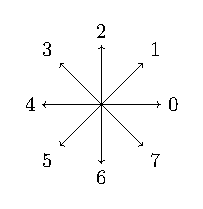
\includegraphics[width=0.3\linewidth]{images/chain-code-dir-num}
    \caption{Example of direction numbers for an 8-directional chain code}
    \label{fig:direction-numbers}
\end{figure}

The code depends on the starting point, but is a circular sequence that can be normalized by letting the starting point be the point that gives the lowest integer value of the sequence. The direction values can also be normalized by using the first difference instead of the absolute direction number.

\subsubsection{Minimum-perimeter polygons (MPPs)}
The goal is to encode the general shape using as few straight segments as possible.

One method is to overlay a coarser grid on the boundary, mark the cells visited by the boundary, and finding the shortest path trough these cells. The hard part is to automate the grid size choice. The algorithm itself is pretty complex stuff.

\subsubsection{Other polygonal approaches}
\paragraph{Merging} This method merges points along a line until the squared sum of errors between the boundary and the line is too large. When the threshold is reached, the procedure repeats with a new line.
\paragraph{Splitting} Start with a line, and find the point that fits the line least. Add that point to the perimeter polygon (now a triangle), and continue until good enough.

\subsubsection{Boundary segments}
It can be useful to separate the boundary into segments. This can be done by finding the convex hull of the shape, and cutting the boundary when it moves in and out of convex deficiencies. See Section \ref{sec:convex-hull}.

For most images, noise etc. will create many small, meaningless convex deficiencies. These can be removed/reduced by smoothing the region, averaging pixels along the boundary, or by using a polygonal approximation.

\subsubsection{Skeletons}
Skeletonizing reduces a shape to a graph, which represents the structural shape of the region. Can be done by thinning (Section \ref{sec:thinning}), but that doesn't ensure connectivity.

The \emph{medial axis transformatian} can be used instead: You have a region $R$ with border $B$. For each point $p \in R$, find its closest neighbor in $B$. If $p$ has more than one such neighbor, it is part of the medial axis. The medial axis then defines the skeleton, which is guaranteed connected. This is computationally heavy to do directly, and there are some more optimized algorithms around.

%%%%%%%%%%%%%%%%%%%%%%%%%%%%%%%%%%%%%%%%%%%%%%%%%%%%%%%%%%%%
\subsection{Boundary descriptors}

\subsubsection{Simple descriptors}
\begin{itemize}
    \item Length: Number of pixels along boundary. For a chain-coded curve: $n\sub{vertical} + n\sub{horizontal} + \sqrt{2} \cdot n\sub{diagonal}$.
    \item Diameter: $\max_{i,j} D(p_i, p_j)$.
\end{itemize}

\subsubsection{Shape numbers}
The shape number of a boundary is the first difference of its chain code, rotated to minimize the integer value. The number of digits of the code defines the order $n$ of the shape number (which is even for a closed boundary).

\subsubsection{Fourier descriptors}
A boundary can be described as a sequence of $K$ points where each point is represented by a complex number:
\begin{equation}
    s(k) = x(k) + \ramuno y(k), \quad k = 0, \dots, K-1
\end{equation}
The DFT and inverse DFT of this is
\begin{equation}
\begin{split}
    a(u) &= \sum_{k=0}^{K-1} s(k) \euler^{- \ramuno 2 \pi \frac{uk}{K}} \\
    s(k) &= \frac{1}{K} \sum_{u=0}^{K-1} a(u) \euler^{\ramuno 2 \pi \frac{uk}{K}}.
\end{split}
\end{equation}
However, if we take the DFT and recreate $s(k)$ with only the first $P$ coefficients, we can get a decent approximation:
\begin{equation}
    \hat{s}(k) = \frac{1}{P} \sum_{u=0}^{P-1} a(u) \euler^{\ramuno 2 \pi \frac{uk}{P}}.
\end{equation}
This is a sort of low-pass filtering. If you simplify to 4 descriptors, you get an ellipse, and with 2 a circle.

\subsubsection{Statistical moments}
Take a boundary segment and rotate it so that the line between its ends is horizontal. The resulting histogram $p(v_i)$ can be described by statistical moments. The mean is
\begin{equation}
    m = \sum_{i=0}^{A-1} v_i p(v_i)
\end{equation}
and the $n$th moment is
\begin{equation}\label{eq:nth-moment}
    \mu_n(v) = \sum_{i=0}^{A-1} (v_i - m)^n p(v_i).
\end{equation}

This essentially describes a boundary as 1D functions.

%%%%%%%%%%%%%%%%%%%%%%%%%%%%%%%%%%%%%%%%%%%%%%%%%%%%%%%%%%%%
\subsection{Regional descriptors}
Regional descriptors are (obviously) used to describe regions rather than boundaries.

\subsubsection{Some simple descriptors}
\begin{itemize}
    \item Area $A$
    \item Perimeter $P$
    \item Compactness $P^2 / A$
    \item Circularity ratio $R_c = 4 \pi A / P^2$
    \item Mean and median intensity
    \item Min and max intensity
    \item Number of pixels over/under mean
\end{itemize}

\subsubsection{Topological descriptors}
Topology is the study of properties unaffected by deformation. Examples are:
\begin{itemize}
    \item The number of holes, $H$.
    \item The number of connected components, $C$.
    \item The \emph{Euler number}, $E = C - H$.
\end{itemize}
We can also extract e.g. the largest connected component of an image.

\subsubsection{Texture}
Textures can be e.g. smooth, coarse, or periodic.

\paragraph{Statistical approaches}
The variance $\sigma^2(z) = \mu_2(z)$ (see \eqref{eq:nth-moment}) is useful, and can be used to define smoothness
\begin{equation}
    R(z) = 1 - \frac{1}{1 + \sigma^2(z)}
\end{equation}
which is $0$ for uniform areas and nearly $1$ for your acne-ridden face.

The 1st (standard deviation), 3rd (histogram skewness), and 4th (relative flatness) moments are also used, and sometimes even higher ones.

Another metric is the \emph{co-occurence matrix} $\M{G} \in \mathbb{Z}^{n \times n}$ for $n$ possible intensity levels. (Group intensities if $\M{G}$ becomes too large.) It is based on a relative position operator, which can be for instance ``one pixel to the right''. Then, if there are, say, 3 occurences of intensity $2$ immediately to the right of intensity $6$, we get $\M{G}_{6,2} = 3$. Then further methods can be used to characterize the co-occurence matrix.

\paragraph{Spectral approaches}
Three Fourier spectrum features are particularly useful:
\begin{itemize}
    \item Prominent peaks give the direction of patterns.
    \item Location of peaks give the spatial period of patterns.
    \item Filtering out periodic features leaves nonperiodic elements which can be analysed statistically
\end{itemize}

To simplify detection and interpretation, you can represent the spectrum in polar coordinates as a function $S(r,\theta)$.

\subsubsection{Moment invariants}
The 2D moment of order $(p+q)$ of an $M \times N$ image is
\begin{equation}
    m_{pq} = \sum_{x=0}^{M-1} \sum_{y=0}^{N-1} x^p y^q f(x,y)
\end{equation}
and the centralized moment is
\begin{equation}
    \mu_{pq} = \sum_{x=0}^{M-1} \sum_{y=0}^{N-1} (x-\bar{x})^p (y-\bar{y})^q f(x,y)
\end{equation}
where
\begin{equation}
    \bar{x} = \frac{m_{10}}{m_{00}}, \quad \bar{y} = \frac{m_{01}}{m_{00}}.
\end{equation}
Then, the \emph{normalized central moments} are
\begin{equation}
    \eta_{pq} = \frac{\mu_{pq}}{\mu_{00}^\gamma} \quad \mbox{with} \quad \gamma = \frac{p+q}{2} + 1
\end{equation}

Based on this, seven moments invariant to translation, scaling, mirroring, and rotation can be formulated. These are the \emph{invariant moments}.

%%%%%%%%%%%%%%%%%%%%%%%%%%%%%%%%%%%%%%%%%%%%%%%%%%%%%%%%%%%%
\subsection[Principal components]{Use of principal components for description}
Principal component analysis is a method of describing data by maximizing variance. The axis that maximizes variance if you project all data points onto it, is the first principal component (PC). That is, the first PC is the axis along which the data is most spread out. All subsequent PCs must be orthogonal to the all other. With many dimensions, you can find $N$ PCs, and describe the data in only those axes. This minimizes the euclidean norm error given the number of axes used.

Each axis is associated with an eigenvalue, and these are nonincreasing from the $n$th to the $(n+1)$th PC. Use this to find which PCs to throw away when you want to reduce dimensionality without damaging the data too much.

\paragraph{Method}
A pixel in an image can be represented as a vector. For an RGB image, this can be $\x = (x_R, x_G, x_B)$. If you gather more data than RGB, the vector will be larger. The mean of all pixel vectors is
\begin{equation}
    \m_{\x} = E\{ \x \} = \frac{1}{K} \sum_{k=1}^K \x_k
\end{equation}
and the covariance is
\begin{equation}
    \M{C}_{\x} = E\left\{ (\x - \m_{\x})(\x - \m_{\x})\T \right\} = \frac{1}{K} \sum_{k=1}^K \x_k \x_k\T - \m_{\x} \m_{\x}\T.
\end{equation}
We can approximate $\x$ by calculating the eigenvectors of $\M{C}_{\x}$, placing them in a matrix $\M{A}$, transforming
\begin{equation}
    \y = \M{A}(\x - \m_{\x}),
\end{equation}
and finally transforming back using a modified $\M{A}$ that only includes the eigenvectors for the $k$ largest eigenvalues:
\begin{equation}
    \hat\x = \M{A}_k\T \y + \m_{\x}
\end{equation}
Then, $\hat\x \in \real{k}$.

%%%%%%%%%%%%%%%%%%%%%%%%%%%%%%%%%%%%%%%%%%%%%%%%%%%%%%%%%%%%
\subsection{Feature parameter fitting using the Hough transform}
The Hough transform can be used to detect and parametrize features such a lines found in an image. It requires an edge image, which can be obtained with e.g. the Canny operator (Section \ref{sssec:adv-edge-detection}). For each edge pixel in the edge image, it loops over parameters for the model, and increments a value for each matching parametrization. The parametrizations with the ``most votes'' will then match features in the image.

A line can be parametrized by two parameters $a$ and $b$
\begin{equation}
    y = mx + b,
\end{equation}
but this gives unbounded $a$, and therefore an unbounded search space of possible parametrizations. Instead, we use the polar parametrization
\begin{equation}
    \rho = x \cos \theta + y \sin \theta,
\end{equation}
where $\rho$ is the shortest distance from the origin to the perpendicular line, and $\theta$ is the angle of the perpendicular, as seen in Figure \ref{fig:polar-line}. Now the parameters are bounded. We can search for any parametrization of a shape, but more parameters require more computation.

\begin{figure}[htbp]
    \centering
    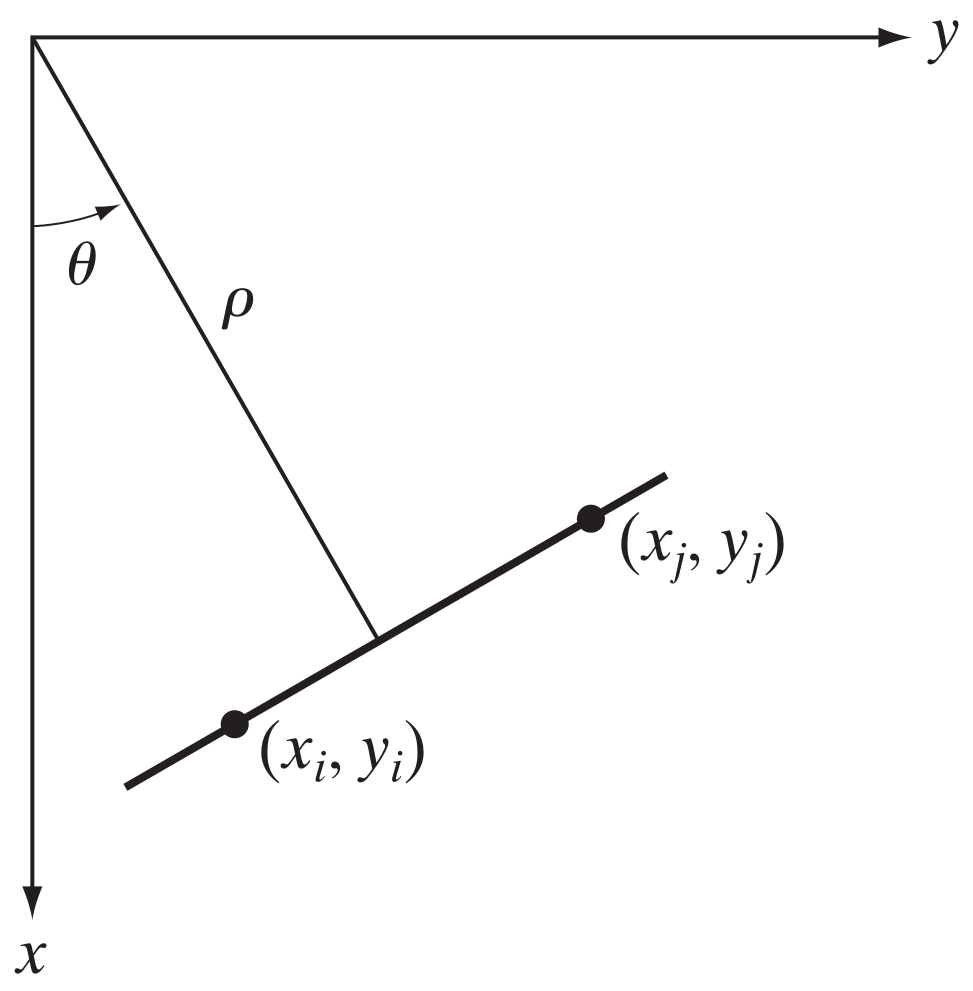
\includegraphics[width=.6\linewidth]{images/R_theta_line}
    \caption{Polar parametrization of a line}
    \label{fig:polar-line}
\end{figure}

%%%%%%%%%%%%%%%%%%%%%%%%%%%%%%%%%%%%%%%%%%%%%%%%%%%%%%%%%%%%
\subsection{Local feature description with SIFT}\label{ssec:sift}
SIFT (scale-invariant feature transform) is an algorithm that detects and describes local features in an image. A rough outline is
\begin{enumerate}
    \item Construct a scale-space: Gaussian-blur the image using increasing $\sigma$ to create a stack of images, ranging from sharp to super blurry. To approximate the LoG, take the difference of each adjacent pair of images. This gives a 3D space in $(x,y,\sigma)$.
    \item Search for local extrema: Max and min values as seen relative to its neighbors in all directions $(x,y,\sigma)$.
    \item Keypoint localization: Use a Taylor series to better find the location of the local extrema. Remove low-contrast keypoints and edge keypoints.
    \item Orientation: Calculate gradient magnitudes in a scale-dependent neighborhood, and put into a gradient histogram. Use this to assign an orientation to the keypoint.
    \item Keypoint descriptor: Use a 16 by 16 neighborhood, divide into 16 blocks, create an 8 bin orientation histogram for each block. You get 128 bin values, which becomes the feature vector of the keypoint.
    \item Matching: Use vector distances to determine matches between descriptors in different images.
\end{enumerate}
